To gain more understanding on the needs, an observation was carried out by the researchers. The reason for choosing this way of data collection is mainly triangulation, which provided us knowledge on the investigated domain from a different angle. On top of that, one of the team members works in an IT office environment in Helsinki, which allowed us to live with this possibility. For sake of confidentiality, the name of the firm and the exact details remain hidden in this report. 

The observation is carried out on a regular workday in the office when most of the employees are present. The room in which the observation is done is shared with four other colleagues. The observed environment is in between a corridor and another room in which other people are working. Therefore, there are multiple people actively working in the room, while occasionally others pass through. Accordingly, the environment is fairly noisy in general and there is some movement and interaction between employees. The room is equipped with rising desks and a whiteboard, that is used for work often by the employees. 

The observed insights and their short descriptions are, as follows:

\begin{enumerate}
	\item \textbf{Arrival to the office}: the first employees started to come around 9 AM and began to work in piece. As more and more people arrived to the office, the level of noise, interaction and movement increased naturally. Typically newcomers greeted their colleagues and initiated casual conversations with fellow coworkers (e.g. by asking how are you today, how was last afternoon, did you get stuck in the traffic as well?). However, some workers just entered the room with a coffee, sat down and began to work. 
	\item \textbf{Meetings}: around 10 AM, some colleagues left for a regular Daily Scrum meeting, which was hosted in another room. Throughout the working days, there are many prescheduled and recurring meetings, which are always hosted in one of the meeting rooms. Others left to their own private meetings/Skype calls during the day so that others are not disturbed and remain focused. In some cases however, people had ad-hoc face-to-face meetings or phone calls in the room which increased the level of noise and disturbance towards others.
	\item \textbf{Noise and interruption}: noise tended to be disturbing in some situations to employees. In most cases once somebody entered the room, he or she began to talk to one of their colleagues which dragged the attention of other workers in the zone. The disturbed employees either joined the conversation (which was either casual or work-related) and changed their attention from their computers to the person who just entered the room. This may or may not be a problem as these interruptions can be constructive to employee relationships or knowledge sharing in the company, but some may consider them as unnecessary interruptions. 	
	\item \textbf{Light in the room}: one interesting observation made during the day was pointed out by one of the employees in the office. Namely, the room has only one window and there is no natural light source coming in from the street. This fact is annoying for employees who work in this room for a long time as days are very short during the Finnish winter and there is not too much natural light whatsoever. For this reason, the company installed a device (similar to the one displayed on Figure \ref{artificial_sunlight}) that provides artificial sunlight that is turned on most of the day. 
	
	\begin{figure}[h] 
		\begin{center}
			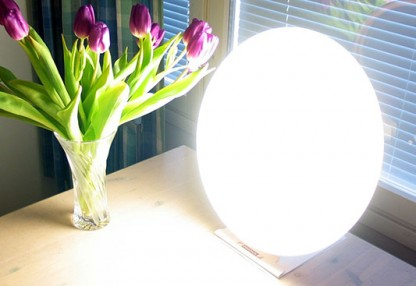
\includegraphics[width=0.9\textwidth]{images/artificial_sunlight.jpg}
			\caption{The office is equipped with a device that provides artificial light to the room with weak access to natural sunlight (the picture is only an illustration).}
			\label{artificial_sunlight}
		\end{center}
	\end{figure}
	\item \textbf{Interaction and breaks}: despite the morning chit-chat and the meetings, colleagues did not interact too much. Mostly, people were into their computers and their work, some even so much that seemingly they did not take any break despite lunch. 
	\pagebreak
	\item \textbf{Cleaning service}: at the end of the day, the cleaners arrived to the office. Their duties during workdays seemed to be limited to gather all glasses and cutlery from the desks of the employees and bring them to the common kitchen on the floor. Seemingly, the only cleaning lady had to make several rounds between the kitchen and the different rooms as the employees left many dishes all around the office. This seemed to be time consuming and probably would have been much faster if the items would be in the kitchen already. 
\end{enumerate}